\section{Transformers}

This section provides an overview of the Transformer model architecture as described by \cite{vaswani2023attention}, later referred to as Vanilla Transformer. This formulation is designed from seq-to-seq tasks and consists of an encoder and a decoder. The encoder maps an input sequence  of embedded representation of words $(x_1, \ldots, x_L)$ to an intermediate representation $(z_1, \ldots, z_L)$. This intermediate representation is then fed to the decoder which then generates the output sequence $(y_1, \dots, y_k)$ one at a time in an auto-regressive manner. Informally, during the optimization process the encoder learns embeddings of the input distribution, while the decoder learns to conditionally generate samples from the desired output distribution.

\begin{figure}[h]
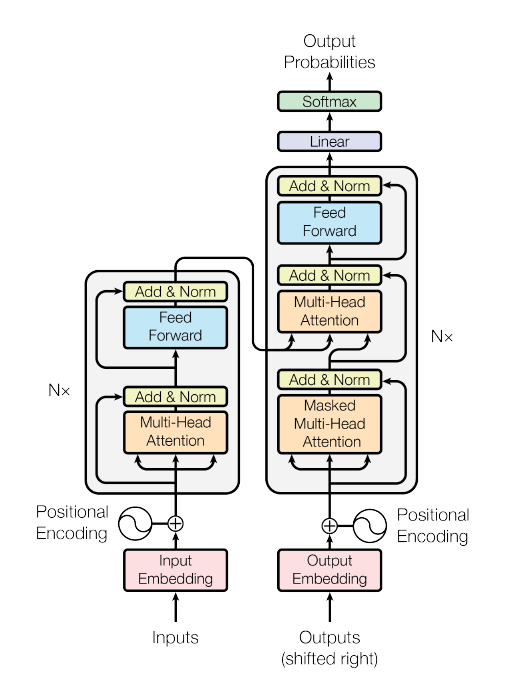
\includegraphics[width=8cm]{images/vanilla-arch.png}
\centering
\caption{Transformers Architecture}
\label{fig:vanilla-arch}
\end{figure}

In order to describe the encoder and decoder of the Transformer architecture, we first need to understand the attention mechanisms and position-wise feed-forward layers.

\subsection{Multi-Head Attention}

Attention is the mechanism used by this architecture to capture dependencies between different positions within a sequence by attending to all positions simultaneously. Mathematically, this is represented by the function 
\begin{equation}
    A(Q, K, V) = \softmax\left(\frac{QK^\top}{\sqrt{d_k}}\right) V,
\end{equation}
$Q \in \mathbb{R}^{m \times d_k}$ is the query matrix, $K \in \mathbb{R}^{n\times d_k}$ is the key matrix, and $V \in \mathbb{R}^{n \times d_k}$ is the value matrix. Indeed, we can think of this 
as responding to a query given a set of key-value pairs by considering the similarity between the queries and the keys and then obtaining the values corresponding to the most similar keys. The product of $QK^T$ is scaled by $1/\sqrt{d_k}$ due to empirical observations that the unormalized operation has values in regions of small gradients for the softmax function.

Additionally, to obtain the matrices $Q, K,$ and $V$, generally an attention mechanism applies a linear map to the inputs $X_Q \in \mathbb{R}^{m \times d}, X_K, X_V \in \mathbb{R}^{n \times d}$, i.e. $Q = X_QW_Q, K=X_KW_K, V=X_VW_V$ for  three learnable matrices $W_Q, W_K \in \mathbb{R}^{d \times d_k}, W_V \in \mathbb{R}^{d \times d_v} $.


What we just described is called an Attention Head and as the name indicates, the multi-headed attention stacks several attention heads with unique sets of parameters in parallel. The outputs $A_1, \ldots, A_h$ of $h$ heads are then concatenated along the embedding dimension. It is convention to set $h = d / d_k$ in order to keep the embedding dimension constant throughout the layers for simplicity to stack.

Multi-head attention has three main variants used for the decoder and encoder:
\begin{enumerate}
    \item \textbf{Self-Attention:} This is the attention block used for the encoder. It sets $X_Q = X_K = X_V = X$, where $X \in \mathbb{R}^{L \times d}$ is the input of the encoder block.
    \item \textbf{Masked Self-Attention:} This is the first attention block used for the decoder. It also has $X_Q = X_K = X_V = X$ where $X \in \mathbb{R}^{k \times d}$ is the input of the decoder block, but in this variant the positions are only allowed to attend to earlier positions in the output sequence. This is done by masking future positions to $-\infty$ before the softmax calculation.
    \item \textbf{Encoder-Decoder Attention:} This is the second attention block used for the decoder. It takes as input $X_Q$ the output of the masked self-attention (after residual connection and normalization as discussed later) and $X_K = X_V = Z$, the output of the encoder stack. This is meant to add the context of the input sequence to the decoder.
\end{enumerate}

\subsection{Position-Wise Feed-Forward Network}

Attached to the output of the attention mechanisms, the Transformer architecture also includes a fully connected feed-forward network applied to each position of the input sequence separately but with the same weights. It consists of two linear layers connected by a ReLU activation. The inner-dimension is denoted by $d_{ff}$ and is generally taken as $d_{ff} = 4d$. It can still be represented by tensordot operations as:
$$
PFFN(X) = ReLU(XW_1 + b_1)W_2 + b_2,
$$ 
Notice that while the attention mechanisms described above capture dependencies between positions, this block embeds positions independently.

\vspace{2em}

As represented in figure \ref{fig:vanilla-arch}, both the encoder and decoder is composed of $N$ layers of identical blocks stacked. Each decoder block consists of a multi-head self-attention mechanism with a residual connector, followed by layer normalization \cite{ba2016layer}, then by a position-wise feed-forward layer also with a residual connector and layer normalization. In a similar manner, a decoder layer 
